\documentclass{article}
\usepackage{graphicx} % Required for inserting images
\usepackage[margin=0.75in]{geometry}
\usepackage{xcolor}
\usepackage{amsmath}
\title{PH.140.644 Note -- In Class}
\author{Moran Guo}
\date{August 2024}

\begin{document}

\maketitle

\section{Aug 29th}
\subsection{Linear Model}
Consider a linear model: $$\hat{f}(X) = \hat{\beta}_0 + \hat{\beta}_1 X + \hat{\beta}_2 X + \hat{\beta}_3 X + \hat{\beta}_4 X + \hat{\beta}_5 X$$

How do we simplify it?\\

1. Sparsity of the parameters: Removing one (or more) variables.\\

2. Use non-linear models to re-model the outcome variable.\\

\noindent Flexibility vs. Interpret-ability\\

Increasing the flexibility \textbf{generalize the model}, but makes the model \textbf{harder to interpret}. -- How do we keep a balance between these two?\\

It seems that methods such as Trees and Generalized Additive Models keep a good balance between these two.\\

\noindent \textbf{Assessing Model Accuracy}\\

We could compute the Avg. MSE over training set ($\mathrm{Tr}$): $$\mathrm{MSE_{Tr}} = \mathrm{Ave_{i \in Tr}}[y_i - \hat{f}(x_i)]^2,$$

but this may be biased toward more over-fit models. Instead, we should use a new test data $\mathrm{Te} = \{x_i, y_i\}_1^M$ and calculate $$\mathrm{MSE_{Te}} = \mathrm{Ave_{i \in Te}}[y_i - \hat{f}(x_i)]^2.$$

In reality, the scenario is much more complex about how to decide the training and testing sets.

(If it's binary or classification problems, we could look at False Negative rate, False Positive rate, or misclassification \%).
\newpage
\begin{figure}[h!]
    \centering
    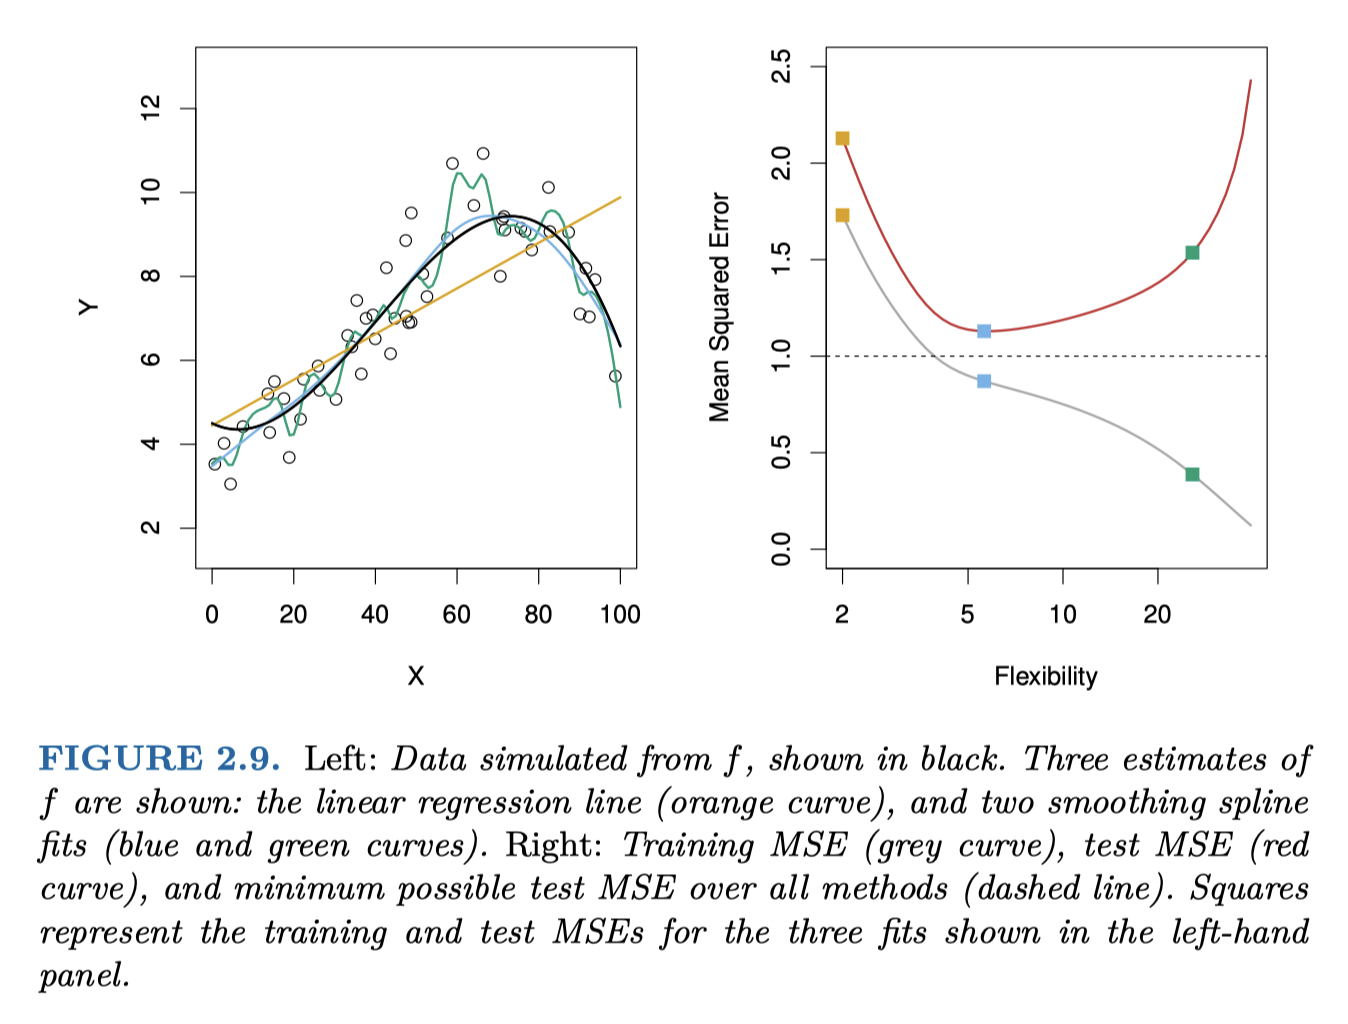
\includegraphics[width=0.75\linewidth]{Training_vs._Testing.png}
    \label{fig:train-vs-test}
\end{figure}

The \textcolor{blue}{blue} smoothing spline fit seems to perform the best across all three models. The \textcolor{green}{green} curve seems to have too much degrees of freedom by increasing the complexity of the model, which over-fits. In reality we are often time observing this U-shaped curve, where the overall MSE decreases when the complexity increase, but when the model is too complex, the $\mathrm{MSE_{Tr}}$ increases.\\

\noindent \textbf{Bias-Variance Trade-off}

Suppose we fit a model $\hat{f}(x)$ to training data $\mathrm{Tr}$, and let $(x_0, y_0)$ be an observation from the population. Then we have $$E\Big(y_0 - \hat{f}(x_0)\Big)^2 = \mathrm{Var}(\hat{f}(x_0)) + \Big[\mathrm{Bias}(\hat{f}(x_0))\Big]^2 + \mathrm{Var}(\epsilon).$$

\begin{figure}[h!]
    \centering
    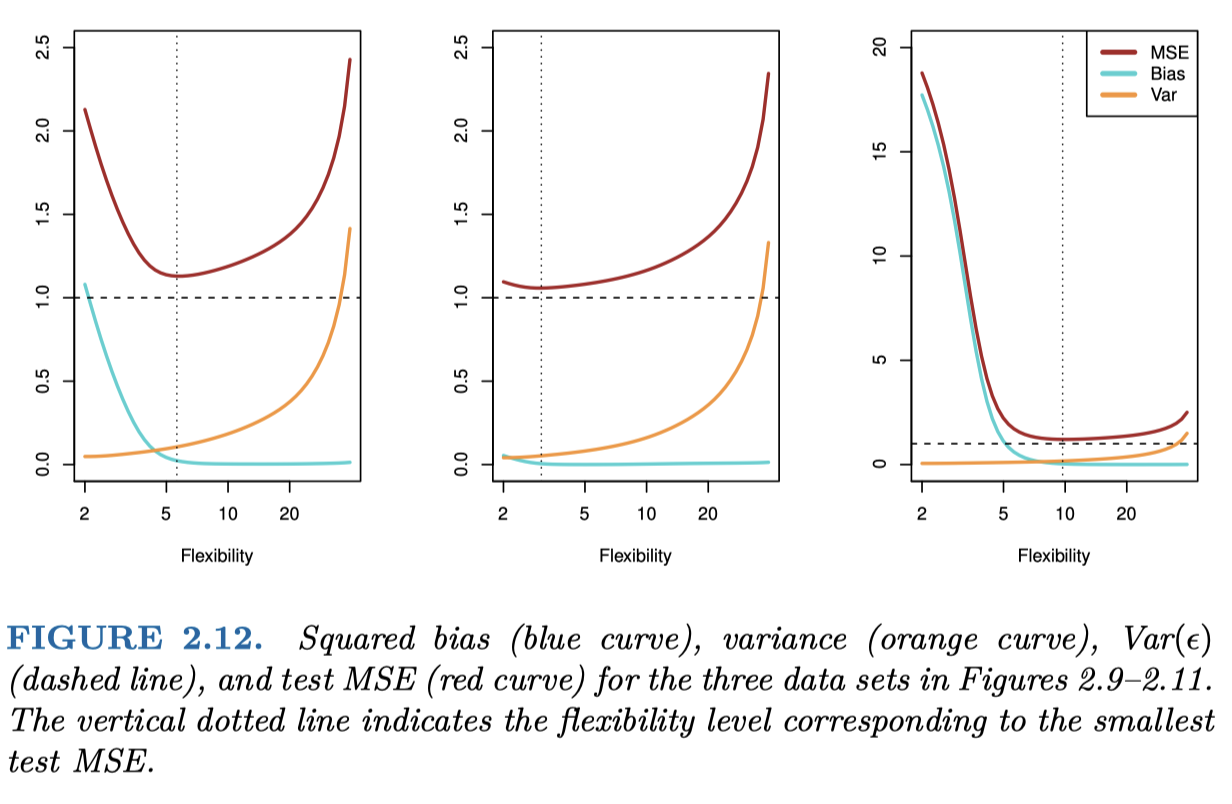
\includegraphics[width=0.75\linewidth]{bias_variance_tradeoff.png}
    \label{Bias-variance-tradeoff}
\end{figure}

As we are using more flexible model, the variance will increase and bias will decrease. But we generally have local minima to find the $\mathrm{MSE_{\min}}$.\\

\noindent \textbf{Classification Problem}

Response variable $Y$ is qualitative. Goal:
\begin{enumerate}
    \item Build a classifier $C(X)$ that assigns a class label from $\mathcal{C}$ to an unlabeled observation $X$.
    \item Assessing the uncertainty in each classification.
    \item Understand the roles of different predictors among $X$.
\end{enumerate}

To find the ideal $C(X)$, for $K$ elements in $\mathcal{C}$ numbered $1, 2, \cdots, K$. Let $$p_k(X) = \mathrm{Pr}(Y=k \vert X = x), k \in [1,K].$$

These are the conditional class probabilities at $x$; Then the \textbf{Bayes optimal classifier} at $x$ is $$C(x) = j$$  if $$p_j(x) = \max\{p_k(x)\}, k \in [1,K].$$\\

Nearest-neighbor averaging can also be used, especially when data is sparse.\\

\noindent \textbf{How good the model is} (classification model)?

Misclassification error rate: $$\mathrm{Err_{Te}} = \mathrm{Ave_{i \in Te}}I[y_i \neq \hat{C}(x_i)]$$

Pay attention to \textbf{selection bias} when having an \textbf{extremely low} misclassification rate.\\

\noindent \textbf{K-nearest Neighbors}
\begin{figure}[h!]
    \centering
    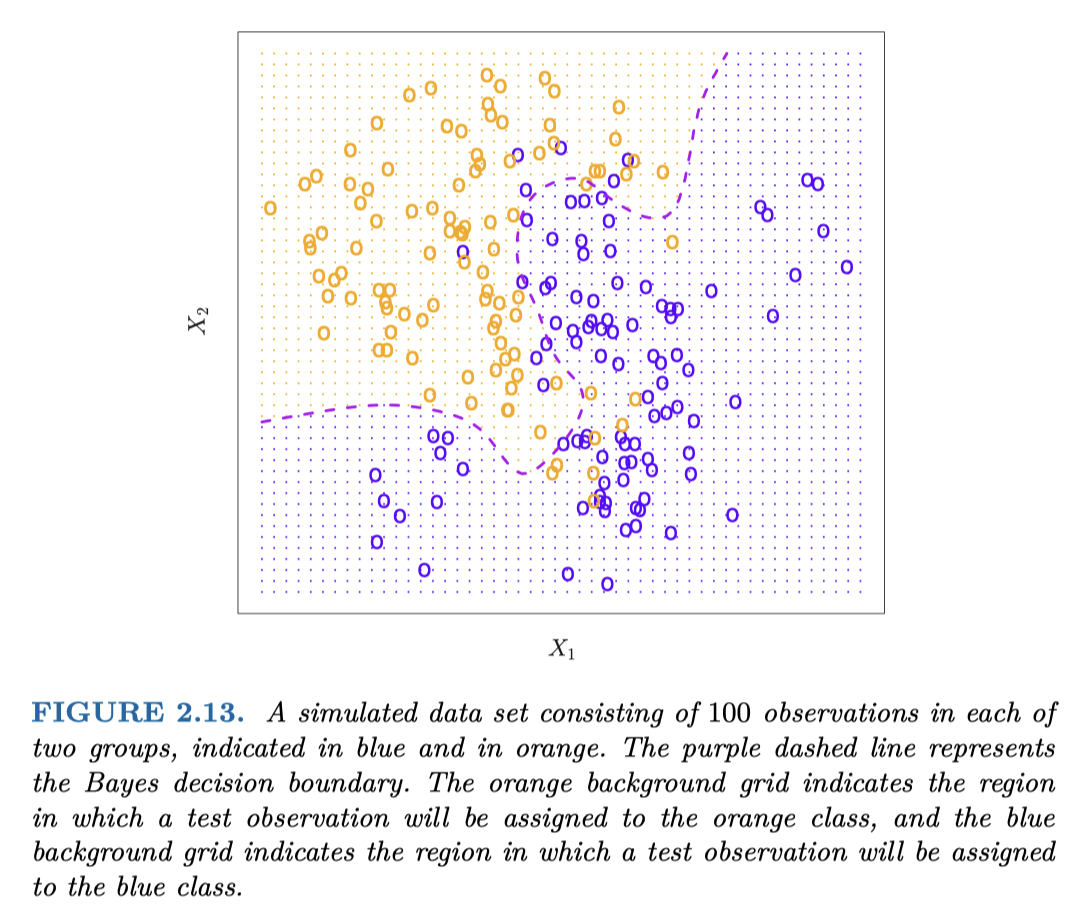
\includegraphics[width=0.60\linewidth]{KNN.png}
    \label{fig:KNN}
\end{figure}

There are some misclassified data which could be observed from the graph.

\newpage

\begin{figure}[h!]
    \centering
    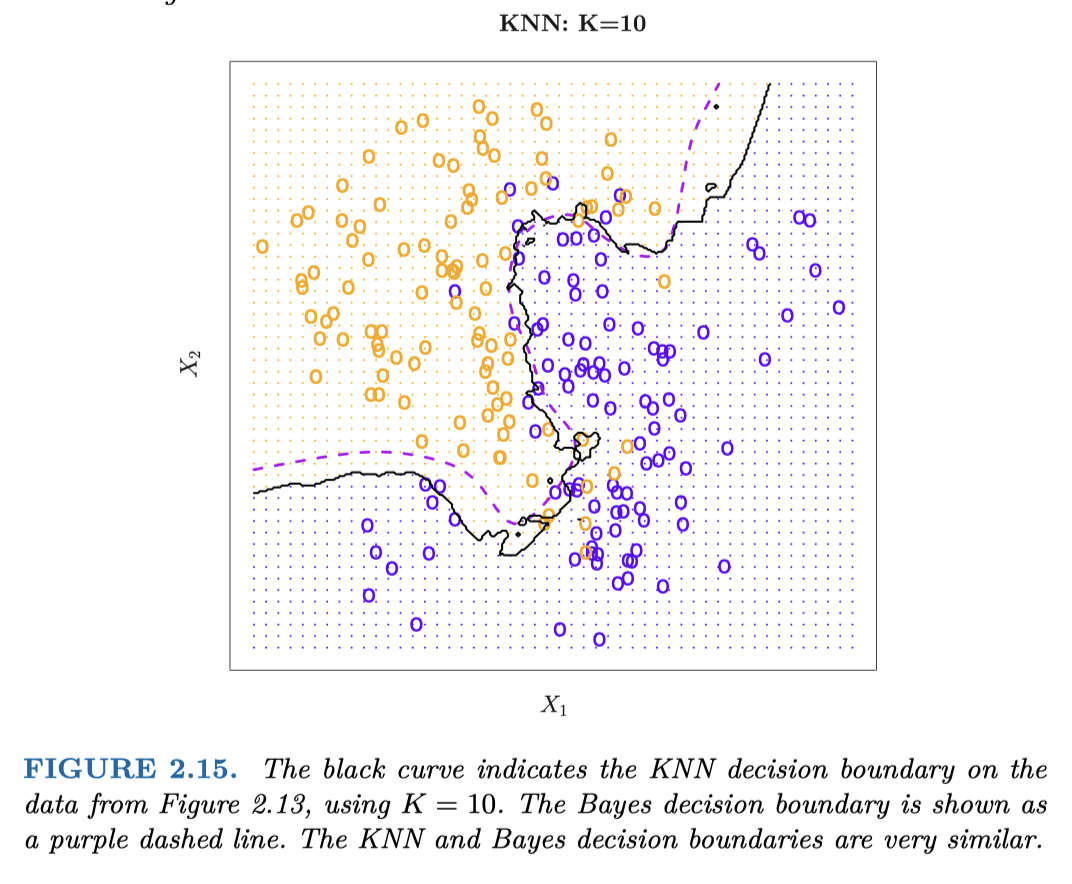
\includegraphics[width=0.5\linewidth]{KNN_10.png}
    \label{fig:KNN-10}
\end{figure}

The black curve is the estimate of the K-Nearest Neighbor with $K = 10$. The boundary is established by sampling the $10$ nearest data points of a particular data point and observe the majority color of those points.

\begin{figure}[h!]
    \centering
    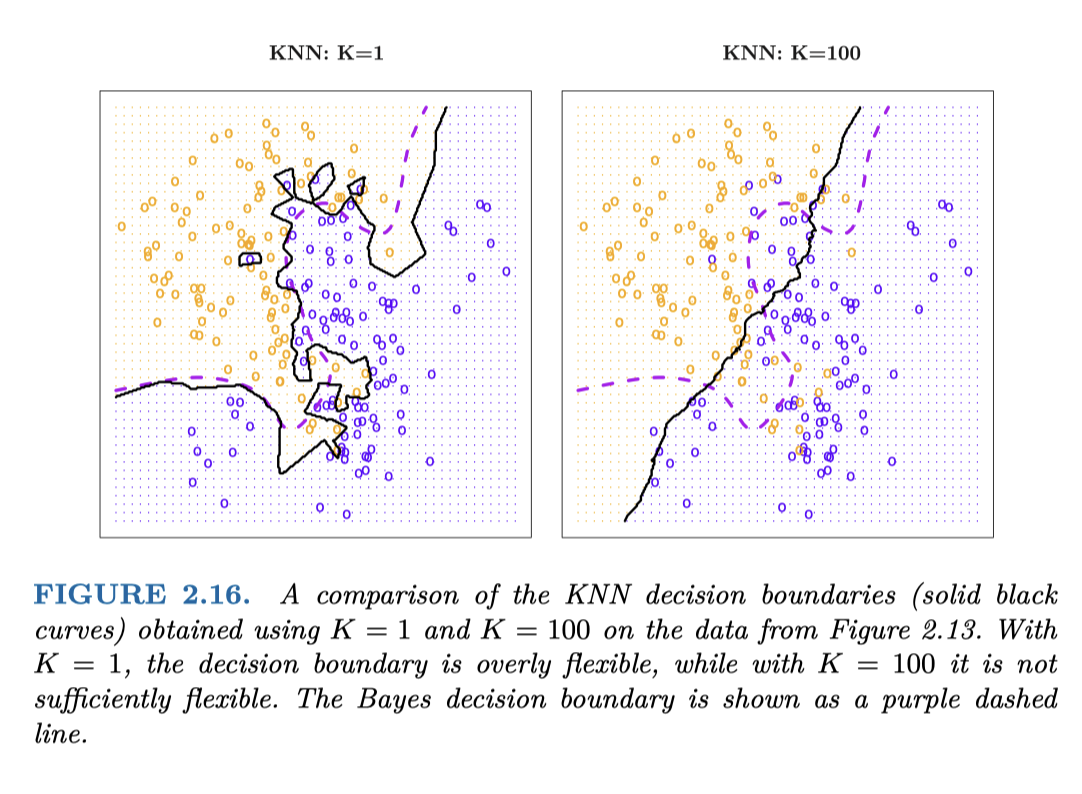
\includegraphics[width=0.75\linewidth]{KNN_compare.png}
    \label{fig:KNN-compare-1-100}
\end{figure}

The $K=1$ KNN estimate gives too much complexity which can be observed from the under-smoothed curve and islands emerged. Instead, if we use $K=100$ KNN, this model gives too little complexity which we cannot learn much from the model.
\newpage
\begin{figure}[h!]
    \centering
    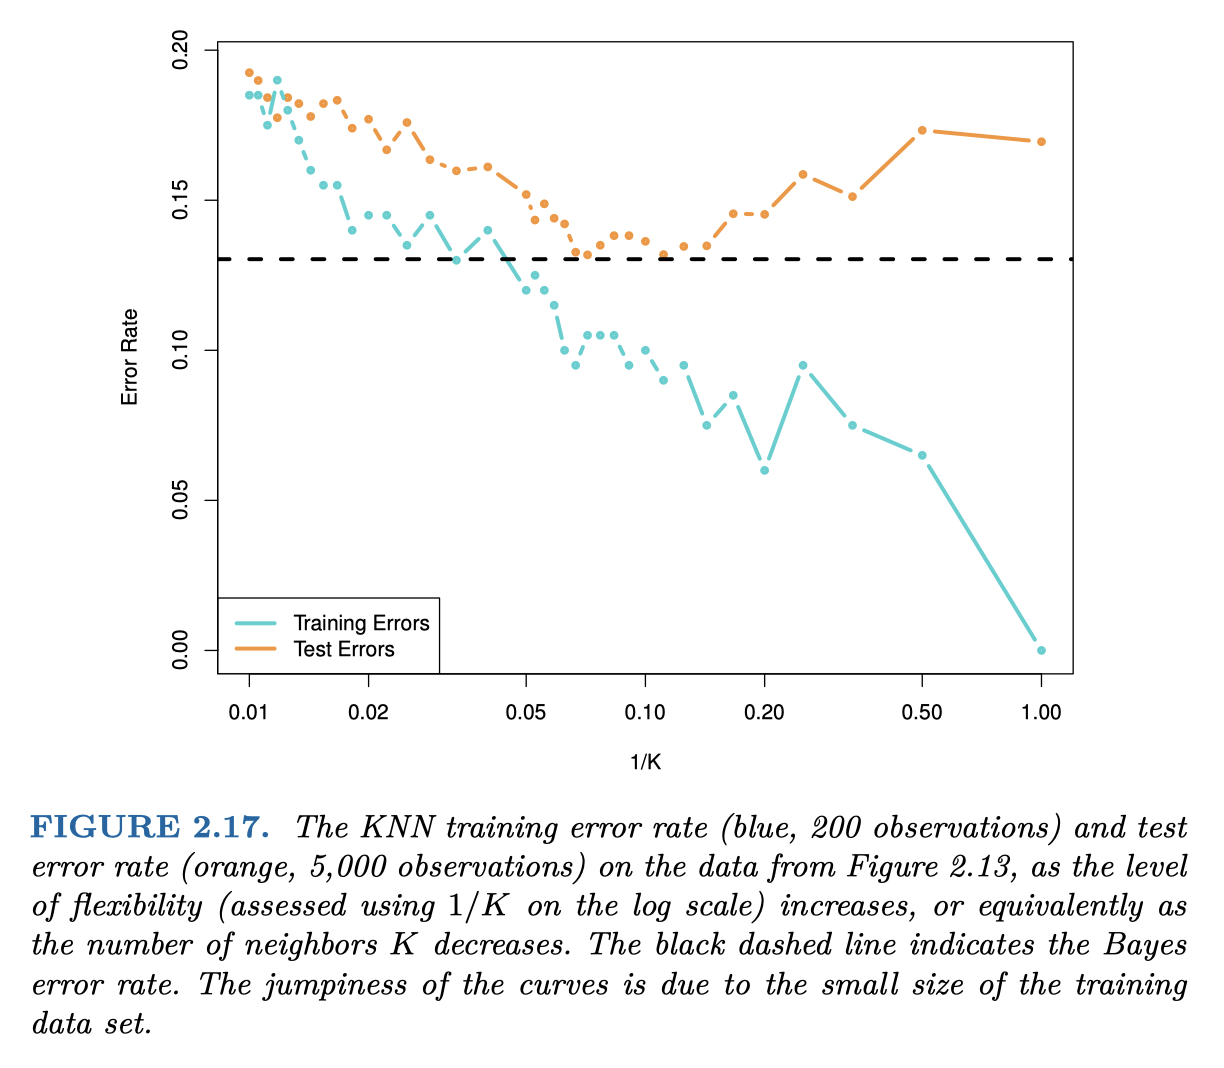
\includegraphics[width=0.75\linewidth]{Training_testing_error.png}
    \label{fig:training-testing-error}
\end{figure}

The training errors goes down as $K$ increases. However, the testing errors generally obey an U-shaped curve. We can see that $K=10$ is optimal here.

\section{Sep 3rd}

\subsection{Linear Regression}

Linear regression is a simple approach to supervised learning. It assumes that the dependence of $Y$ on $X_1, X_2, \dots, X_p$.\\

\noindent \textbf{Variable Selection}\\

Strategy 1:
Try one variable at a time, and calculate the training error.\\

For multiple variables, we consider \textit{all subsets} of the variables to select the \textbf{best} \textit{subset} of the combination of variables. However, there are too much $(2^p)$ of combinations, so it is not realistic.\\

So we need an automated approach that searches through a subset of them. (Refer to book pp. 79)

\subsection{Classification}

Qualitative variables in an unordered set $\mathcal{C}$, e.g., eye color, email, etc.\\

Given: feature vector $X$ and qualitative response $Y$ taking values from $\mathcal{C}$, classification is to:\\

Build a function $C(X)$ s.t. takes feature vector $X$ as input and output predicted $Y$.

\newpage

\begin{figure}[h!]
    \centering
    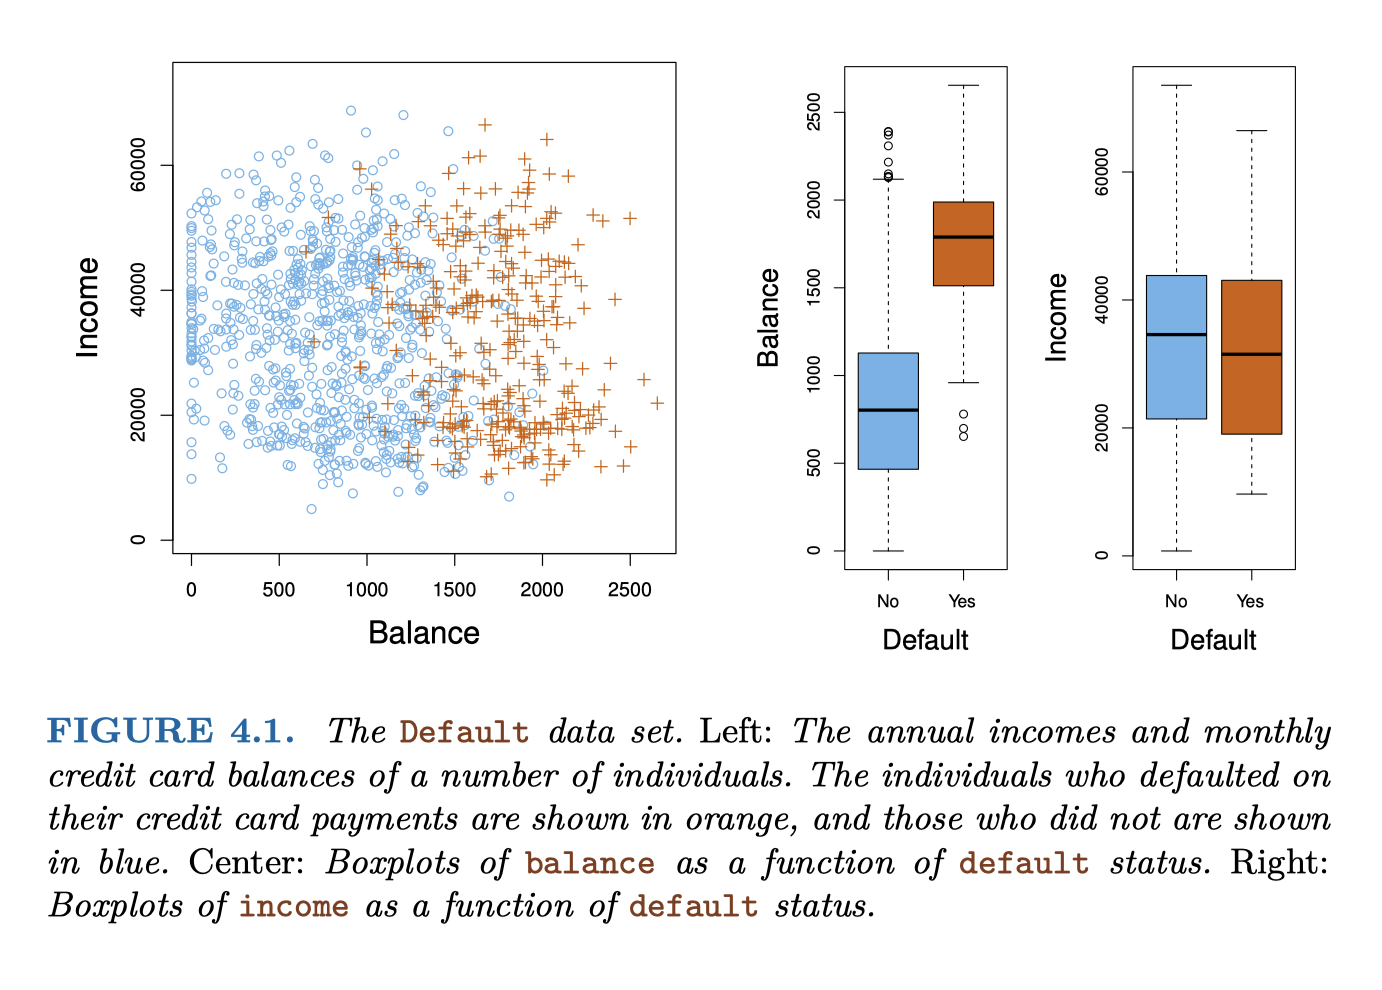
\includegraphics[width=0.75\linewidth]{Classification_income_vs_balance.png}
    \label{fig:income-vs-balance}
\end{figure}

Clients that have a high balance are associated with higher chance (observed) of default, compared to those with a low balance.\\

Can we perform a simple linear regression to predict a binary outcome?
E.g., perform a regression of $Y$ on $X$ and classify as ``Yes'' (or ``No'') if $\hat{Y} > 0.5$? -- Yes we can.\\

However, linear regression does not provide meaningful estimates of $\mathrm{Pr}(Y \vert X)$, compared to logistic regression.

\subsection{Logistic Regression}

$p(X) = \mathrm{Pr}(Y = 1 \vert X)$, consider using $\color{red}{balance}$ to predict $\color{red}{default}$. Logistic regression uses $$p(X) = \frac{e^{\beta_0 + \beta_1 x}}{1 + e^{\beta_0 + \beta_1 x}} \Longrightarrow \frac{p(X)}{1-p(X)} = e^{\beta_0 + \beta_1 x}.$$

$\displaystyle \frac{p(X)}{1 - p(X)}$ is called \textbf{odds}.\\

We uses Maximum Likelihoods to estimate the parameters:

$$\displaystyle\ell(\beta_0, \beta_1) = \prod_{i:y_i = 1}p(x_i)\prod_{i:y_i = 0}\Big(1 - p(x_i)\Big)$$

\begin{figure}[h!]
    \centering
    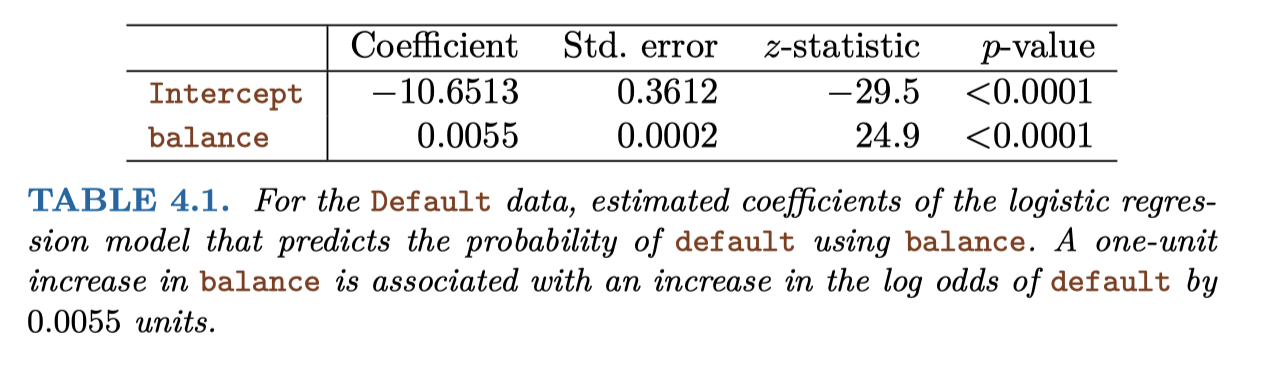
\includegraphics[width=0.75\linewidth]{GLM_result.png}
    \label{GLM-logistic}
\end{figure}

We can start to make a prediction now. From the table above we get $\hat{\beta}_0 = -10.6513$ and $\hat{\beta}_1 = 0.0055$. So 

\newpage

\begin{figure}
    \centering
    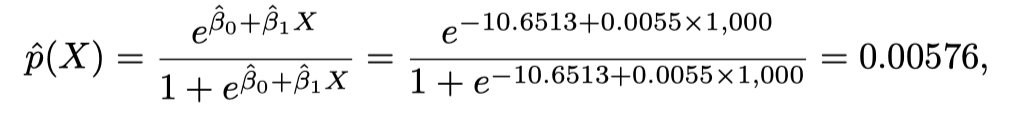
\includegraphics[width=0.75\linewidth]{calculation_logistic.png}
    \label{calculation-logistic}
\end{figure}

with a balance of $\$1000$.

\subsection{Confounding}

\subsection{Multiple Logistic Regression}

$$\mathrm{Pr}(Y = k \vert X = x) = \frac{e^{\beta_{k0} + \beta_{k1} + \dots + \beta_{kp}x_p}}{1 + \sum_{l=1}^{K=1}e^{\beta_{l0} + \beta_{l1x_1} + \dots + \beta_{lp x_p}}}$$

To predict the most likely class for multiple classes.

\subsection{Discriminant Analysis}

The approach is to model the distribution of $X$ in each of the class separately, then uses $\color{green}{\mathrm{Bayes \ Theorem}}$ to obtain $\mathrm{Pr}(Y \vert X)$.

$$\mathrm{Pr}(Y = k \vert X = x) = \frac{\mathrm{Pr}(X = x \ \vert\ Y = k) \cdot \mathrm{Pr}(Y = k)}{\mathrm{Pr}(X = x)}$$

Note that the denominator is \textbf{not dependent on} $k$.\\

For discriminant analysis we write 
$$\mathrm{Pr}(Y = k \vert X = x) = \frac{\pi_k f_k(x)}{\sum_{l=1}^K \pi_l f_l(x)}$$

Why discriminant analysis?\\

The logistic regression model are \textbf{unstable when the classes are well-separated}. Linear discriminant analysis does not suffer from this problem.\\

If $n$ is small and the distribution of the predictors $X$ is approx. normal in every classes, then the linear discriminant model is more stable than the logistic regression model.\\

Also, it is popular when we have more than two response classes.\\

\textbf{Linear Discriminant Analysis when $p = 1$}

From Gaussian density, $$f_k(x) = \frac{1}{\sqrt{2\pi}\sigma_k}e^{-\frac{1}{2}\Big(\frac{x - \mu_k}{\sigma_k}\Big)^2}$$

We assume that all the $\sigma_1 = \sigma_2 = \dots = \sigma_k$.

Then we find that $$p_k(x) = \frac{\pi_k \frac{1}{\sqrt{2\pi}\sigma}e^{\Big(- \frac{1}{2\sigma^2}(x - \mu_k)^2\Big)}}{\sum_{l=1}^K \pi_l \frac{1}{\sqrt{2\pi}\sigma}e^{\Big(- \frac{1}{2\sigma^2}(x - \mu_l)^2\Big)}}.$$

\section{Sep 5th}

\textit{Control the size of the submitted PDF file.}

\subsection{Estimate the parameters}
Start from 
$$\mathrm{Pr}(Y = k \vert X = x) = \frac{\pi_k f_k(x)}{\sum_{l=1}^K \pi_l f_l(x)}$$

We estimate $\displaystyle\hat{\pi}_k = \frac{n_k}{n}$, $\displaystyle\hat{\mu}_k = \frac{1}{n_k}\sum_{i: y_i = k}x_i$, $\displaystyle\hat{\sigma}^2 = \frac{1}{n - K}\sum_{k=1}^K \sum_{i: y_i = k}(x_i - \hat{\mu}_k)^2 = \sum_{k=1}^K \frac{n_k -1}{n - K}\cdot \hat{\sigma}_k^2.$\\

We are trying to ask the question ``is this subject looks more alike a subject who didn't defaulted or did defaulted?''

\subsection{LDA with $p$-dimensional $(p > 1)$}

From the multivariate Gaussian density:

\begin{figure}[h!]
    \centering
    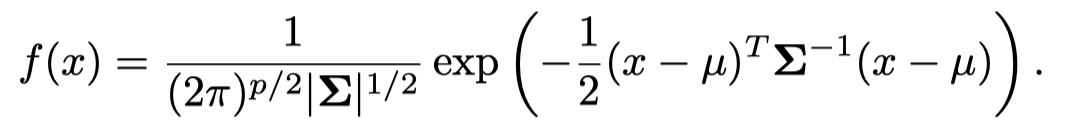
\includegraphics[width=0.75\linewidth]{Multi_Gaussian.png}
    \label{multi_gaussian}
\end{figure}

We construct the Bayes classifier as $$\delta_k(x) = x^T \Sigma^{-1}\mu_k - \frac{1}{2}\mu_k^T \Sigma^{-1}\mu_k + \log \pi_k$$

$\delta_k(x)$ is a linear function despite its complex form.

\begin{figure}[h!]
    \centering
    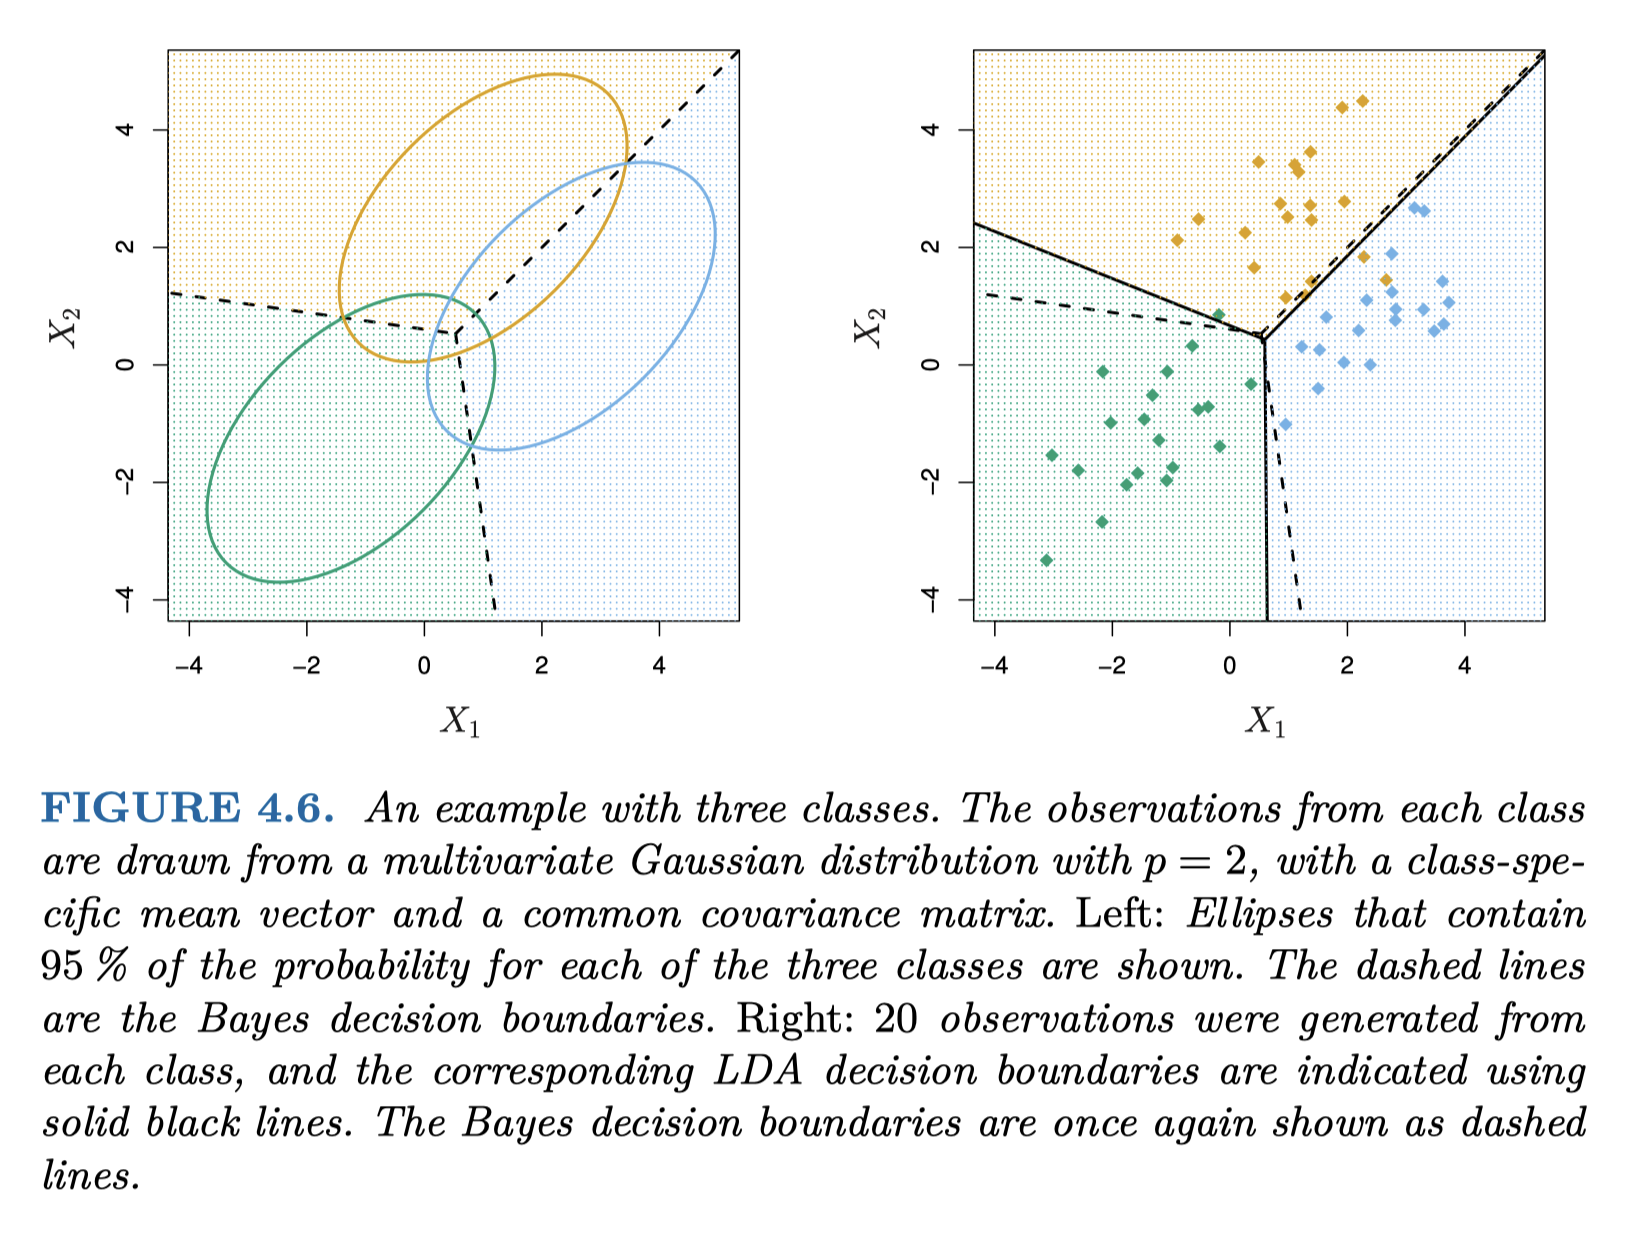
\includegraphics[width=0.75\linewidth]{Bayes_boundaries.png}
    \label{Bayes_boundaries}
\end{figure}

Deviations between the true and estimated Bayes classifier boundaries exist. Dashed lines indicate the Bayes decision boundaries.

\newpage

\begin{figure}
    \centering
    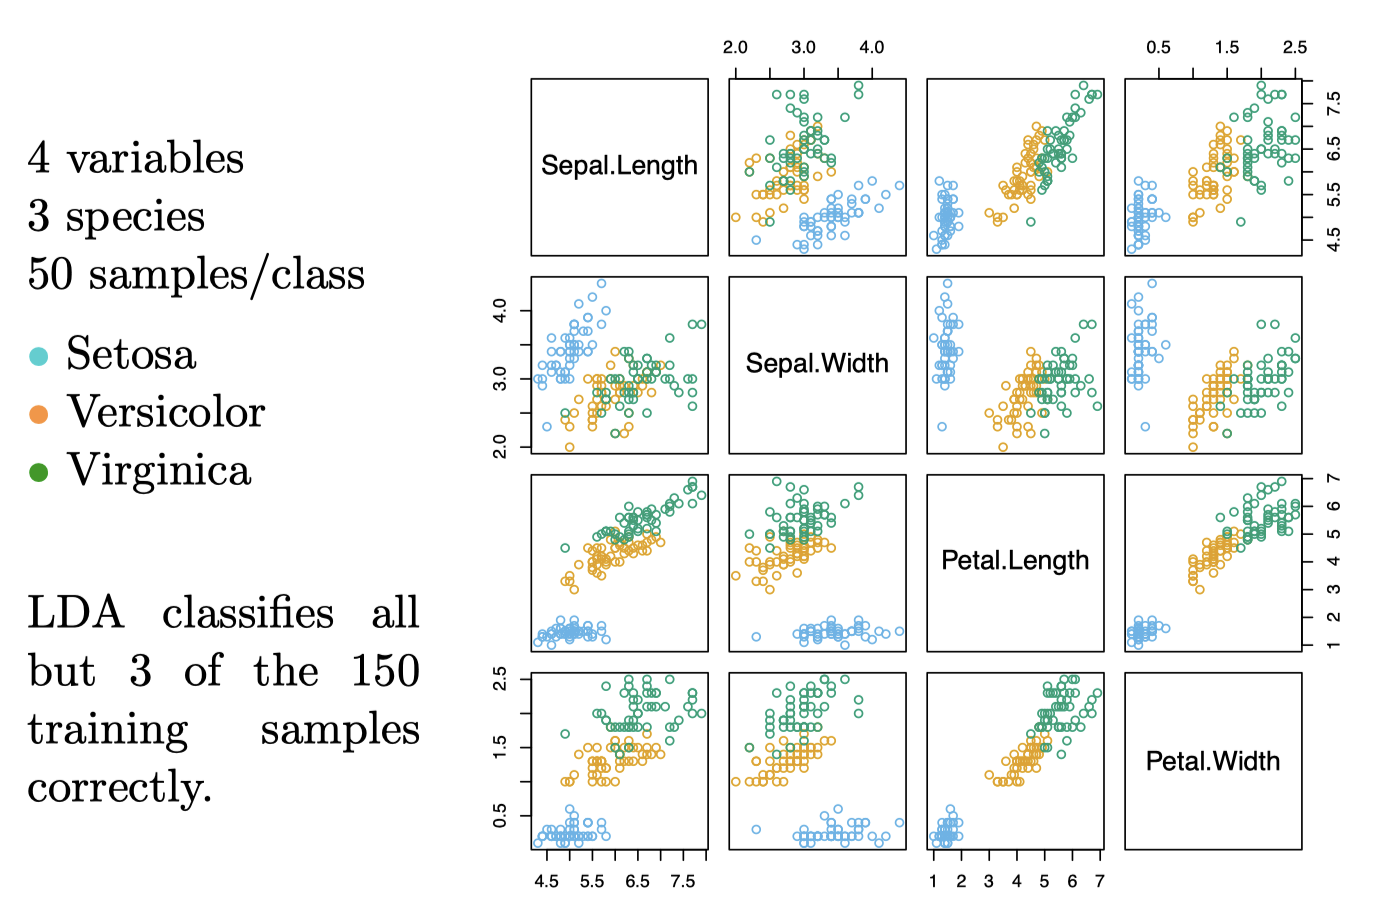
\includegraphics[width=0.75\linewidth]{Iris_data.png}
    \label{Iris_data}
\end{figure}

From the figure, we can observe that $\color{blue}{Setosa}$ species separate well compared to the rest two species.

\begin{figure}[h!]
    \centering
    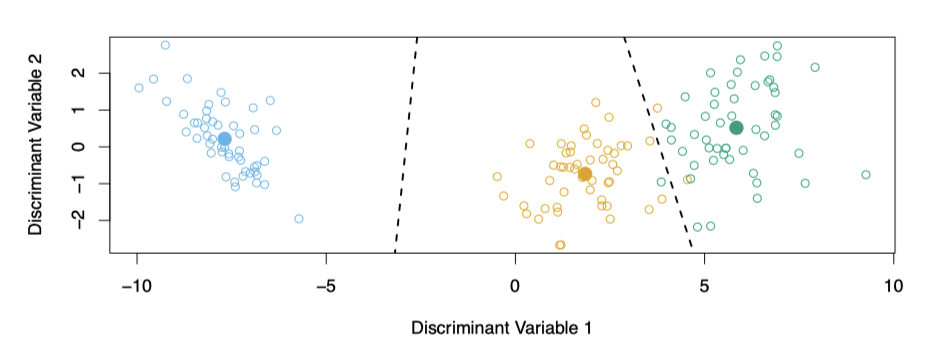
\includegraphics[width=0.75\linewidth]{Discriminant_plot.png}
    \label{Discriminant_plot}
\end{figure}

From the data, we first calculate \textbf{Discriminant Variable} $1$ and $2$ from the variables of the data provided. Then we plot them on the Fisher's discriminant plot and assign to specific classes.

From $\hat{\delta}_k(x)$ we can turn these into estimates of probabilities: $$\widehat{\mathrm{Pr}}(Y = k \vert X = x) = \frac{e^{\hat{\delta}_k(x)}}{\sum_{l=1}^K e^{\hat{\delta}_l(x)}}.$$
\newpage
\begin{figure}[h!]
    \centering
    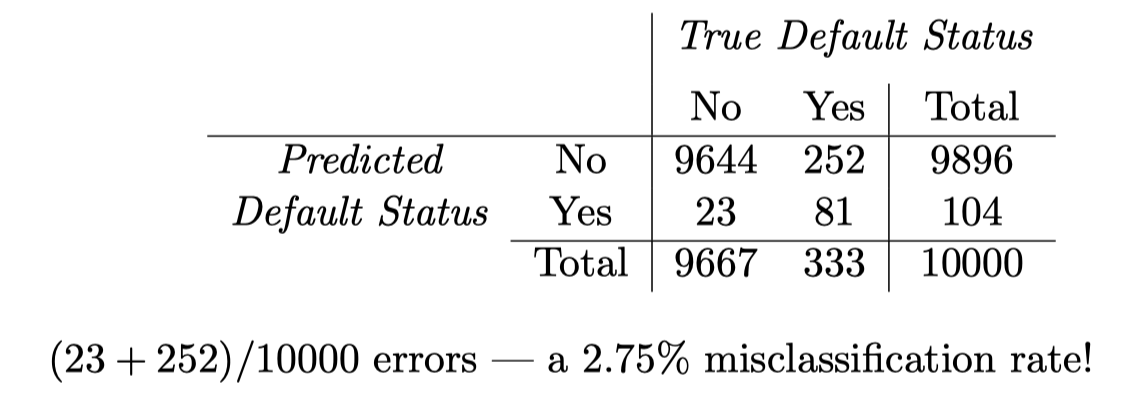
\includegraphics[width=0.75\linewidth]{Credit_data_LDA.png}
    \label{Credit_data_LDA}
\end{figure}

From the example, we have a $2.75\%$ misclassification rate.\\

Caveats:
\begin{enumerate}
    \item This is training error, may be overfitting.
    \item Notice the inbalance of the data. If we always classifies the data into ``non-default'' category, we only have a $3.33\%$ error rate.
    \item Among the 333 cases that are truly default, the model wrongly predicted a large majority of the cases $(252/333 = 75.7\%)$ as being not default. This is a high false negative rate.
\end{enumerate}

\begin{figure}[h!]
    \centering
    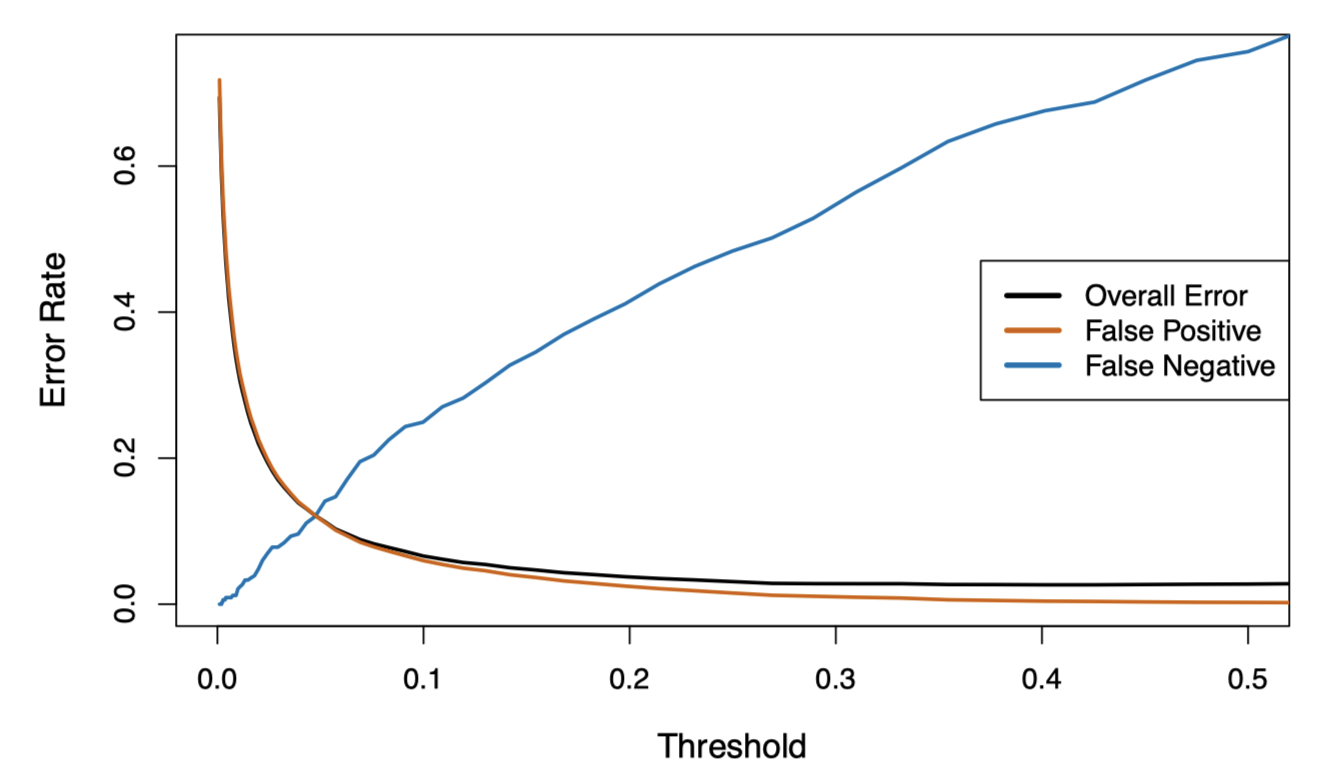
\includegraphics[width=0.75\linewidth]{FN_FP_tradeoff.png}
    \label{FN_FP_tradeoff}
\end{figure}

There is always a trade-off between reducing false negative and false positive rate. If we want to reduce one, the other will increase.

\newpage

\subsection{ROC Curve}

\begin{figure}[h!]
    \centering
    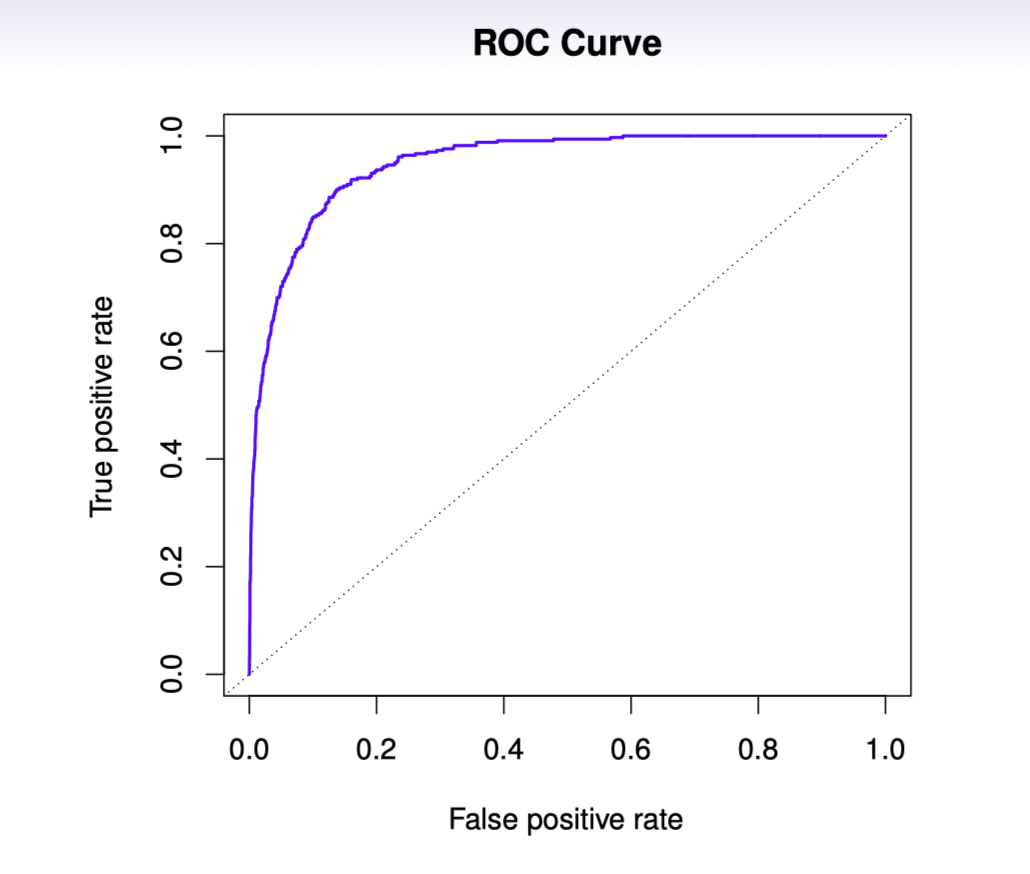
\includegraphics[width=0.5\linewidth]{ROC.png}
    \label{ROC}
\end{figure}

ROC curve allows for plotting false positive and true positive rates on the same plot and thus allows us to determine a \textit{threshold}. Sometimes we use \textit{AUC} (area under the curve) to evaluate the performance of the model, with the higher \textit{AUC} the better the performance.

\section{Sep 10th}
\subsection{Other forms of Discriminant Analysis}

\textbf{Quadratic Discriminant Analysis}: assumes that each class has its own covariance matrix. It assumes that an observation from the \textit{k}th class is of the form $X \sim N(\mu_k, \boldsymbol{\Sigma}_k)$. So we have the Bayes classifier assigns an observation $X = x$ such that 
\begin{figure}[h!]
    \centering
    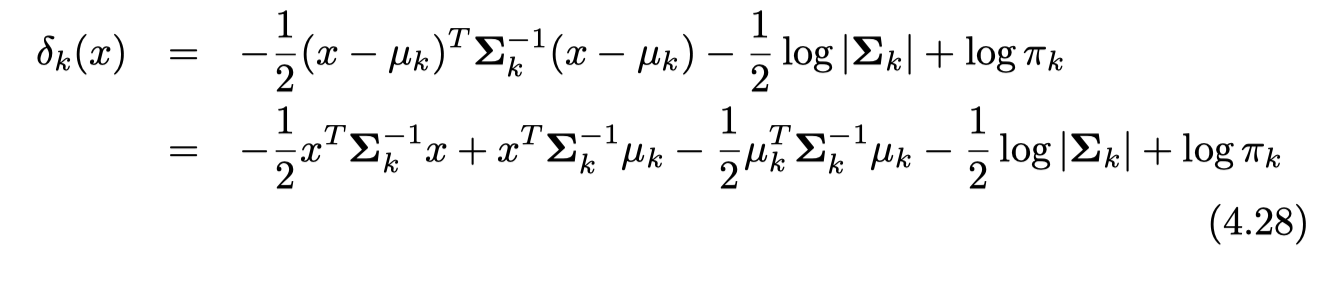
\includegraphics[width=0.75\linewidth]{QDA.png}
\end{figure}
\begin{figure}[h!]
    \centering
    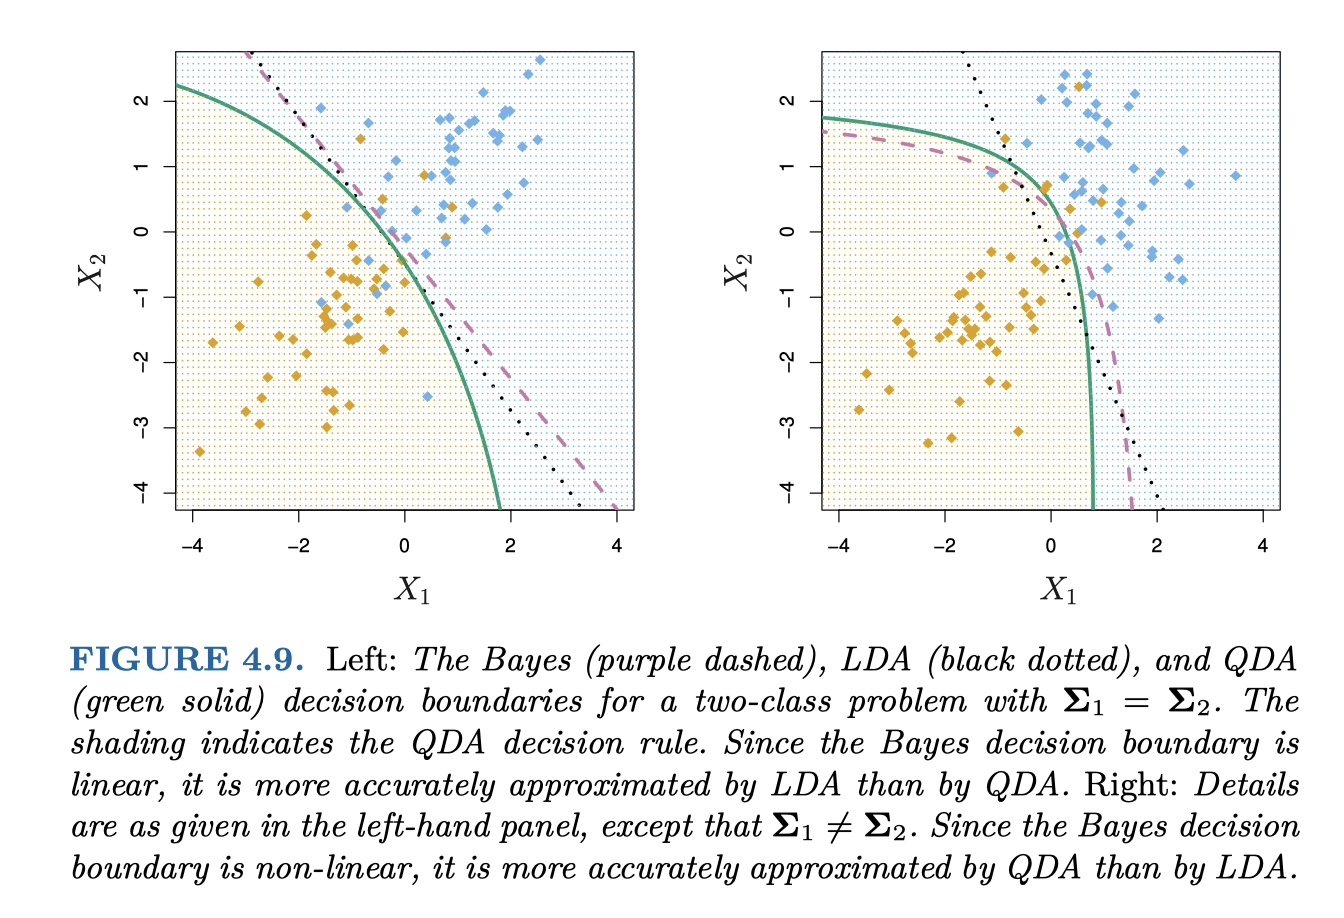
\includegraphics[width=0.5\linewidth]{QDA_fig.png}
\end{figure}

QDA performs better when the Bayes decision boundary is non-linear.\\

\noindent\textbf{Naive Bayes}: with $\displaystyle f_k(x) = \prod_{j=1}^p f_{jk}(x_j)$ (conditional independence model) in each class we have naive Bayes. Assumes features are independent in each class. Useful when \textit{p} is large. Gaussian Naive Bayes assumes each $\boldsymbol{\Sigma}_k$ is diagonal:

\begin{figure}[h!]
    \centering
    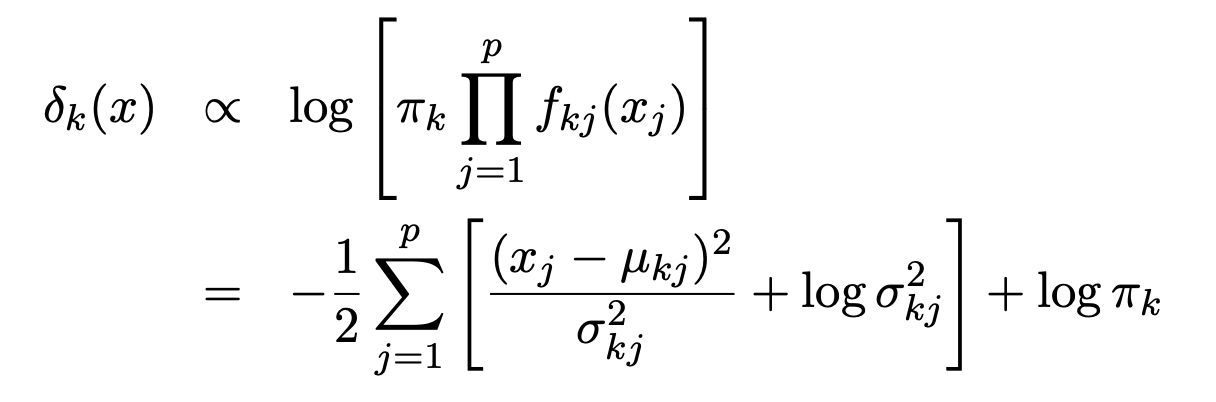
\includegraphics[width=0.75\linewidth]{Naive_bayes.png}
\end{figure}

Can be used for mixed feature vectors, like a mix of qualitative and quantitative. For qualitative, replace $f_{kj}(x_j)$ with probability mass function.

\subsection{Linear Regression vs. LDA}

For a two class problem, we can trivially show that $$
\log\Big(\frac{p_1(x)}{1 - p_1(x)}\Big) = \log\Big(\frac{p_1(x)}{p_2(x)}\Big) = c_0 + c_1 x_1 + \dots + c_p x_p$$

So two-class LDA and logistic regression have the same form. Difference resides in the way that parameters are estimated:

\begin{itemize}
    \item Logistic regression uses the conditional likelihood based on $\mathrm{Pr}(Y \vert X)$, or discriminative learning.
    \item LDA uses the full likelihood based on $\mathrm{Pr}(X, Y)$, or generative learning.
    
\end{itemize}

\section{Cross-Validation \& Bootstrap (Resampling)}

\begin{figure}[h!]
    \centering
    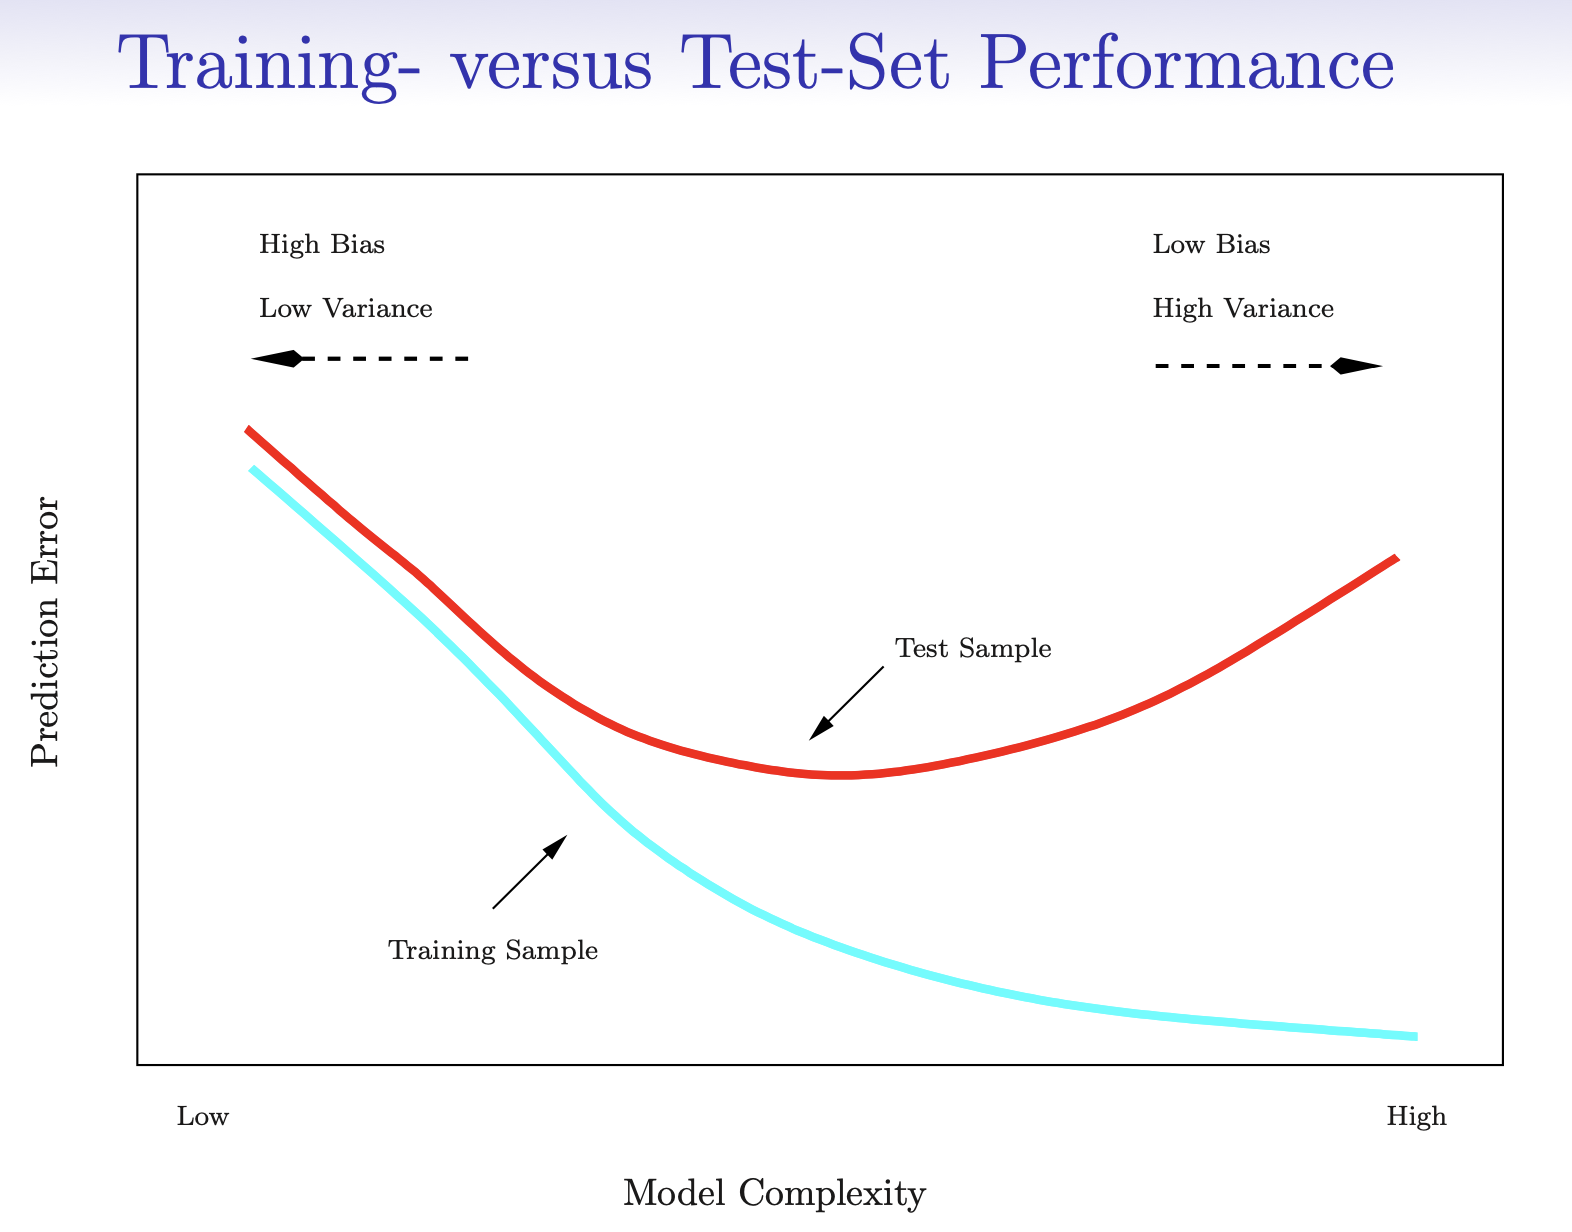
\includegraphics[width=0.5\linewidth]{Error_vs_complexity.png}
\end{figure}

As the model complexity increase, the training sample error generally goes down, but the testing sample error is U shape, thus underfitting or overfitting may negatively affect (increase) the error on the testing data.\\

Here, we consider a class of method that estimate the test error by \textit{holding out} a subset of the training observation from the fitting process.

\subsection{Validation set approach}

We randomly divide the available set of samples into a \textit{training set} and a \textit{validation set}. The model is fitted on the training set, and the fitted model is used to predict the responses for the observation in the validation set.

\subsection{\textit{K}-fold CV}

A \textit{widely used approach} for estimating test error.\\

Idea is to randomly divide the data into \textit{K} equal-sized parts (E.g., $K = 10$ or $K = 5$), then assign one part as validation set, the rest as train set. This process is repeated for exactly $K$ times.

Denote the $K$ parts by $C_1, C_2, \dots, C_K$, then we can compute $$\mathrm{CV}_{(K)} = \sum_{k=1}^K \frac{n_K}{n}\mathrm{MSE}_k$$ where $\displaystyle \mathrm{MSE}_k = \sum_{i\in C_k}\frac{(y_i - \hat{y}_i)^2}{n_k}$, and $\hat{y}_i$ is the fit for observation $i$. Setting $K = n$ yields $n$-fold or leave-one-out CV.


\section{Sep 12th}

$K$-fold CV is not repeated. We only execute it for one time. Since sets are assigned randomly, to account for the randomness, we need to execute this process for multiple times (E.g., Monte Carlo, Repeated $K$-fold CV, etc.).

\subsection{CV for Classification}

$$\mathrm{CV}_k = \sum_{k=1}^K \frac{n_k}{n} \mathrm{Err}_k, \text{ where } \mathrm{Err}_k = \sum_{i \in C_k} I(y_i \neq \hat{y}_i)/n_k. $$

Estimated standard deviation $\displaystyle \mathrm{\widehat{SE}}(\mathrm{CV}_K) = \sqrt{\sum_{k=1}^K (\mathrm{Err}_k - \overline{\mathrm{Err}_k})^2/(K-1)}.$

\begin{figure}[h!]
    \centering
    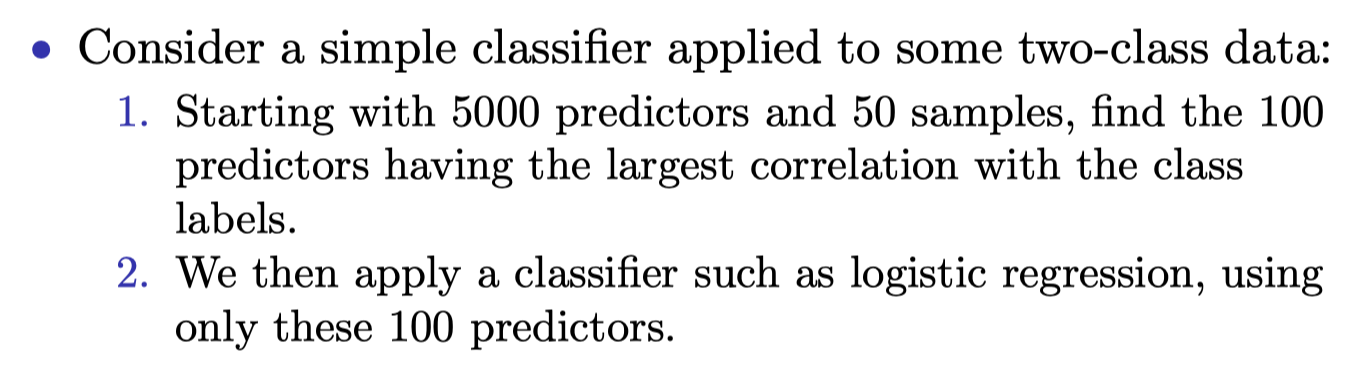
\includegraphics[width=0.90\linewidth]{exmaple_case.png}
\end{figure}

What is the correct way? Step 1 already exposes the data, or the procedure has already seen the labels of the training data. It is \textbf{wrong} to apply CV in step 2 only. The correct way is to apply CV to both step 1 \& 2. CV need to be applied to both training and test set, well before doing anything else.

For bootstrapping multiple times, 

\subsection{Bootstrap}

Used to quantify the uncertainty associated with a given estimator.\\

How bootstrap works?\\

E.g. 

\begin{figure}[h!]
    \centering
    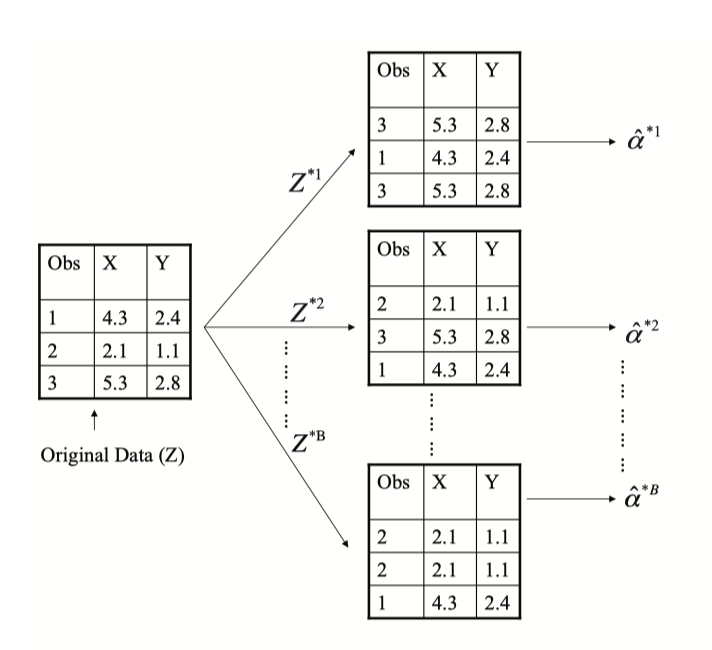
\includegraphics[width=0.5\linewidth]{bootstrap.png}
\end{figure}

Bootstrap is \textbf{sampling with replacement.} For a small sample size containing $n = 3$ observations, each bootstrap data set contains $n$ observations (sampled with replacement). Each bootstrapped data set gives an estimate of $\alpha$. We denote these $\alpha$'s as $\hat{\alpha}^{*1}, \hat{\alpha}^{*2}, \dots, \hat{\alpha}^{*B}.$ We estimate the standard error of the bootstrapped data set by $$
\mathrm{S E}_{B} ( \hat{\alpha} )=\sqrt{\frac{1} {B-1} \sum_{r=1}^{B} \left( \hat{\alpha}^{* r}-\bar{\hat{\alpha}}^{*} \right)^{2}}. 
$$

This serves as an estimate of the standard error of $\hat{\alpha}$ estimated from the original data set. Bootstrap has some drawbacks, like it cannot be used to analyze time series data.\\

\noindent \textbf{Can the bootstrap estimate prediction error?}
\\

In CV, each of the $K$ validation folds is distinct (\textbf{no overlap}) used for training. But bootstrap data must and will have a significant overlap (about 2/3) of the data. This causes it to seriously underestimate the true prediction error.

\subsection{More general non-linear models}

\textbf{Subset selection}\\

How to decide what is the best? Let $\mathcal{M}_0$ denote the null model, which contains no predictors. This model simply predicts the sample mean for each observation.\\

For $k = 1, 2, \dots, p:$\\
(a) Fit all $p \choose k$ models that contain exactly $k$ predictors.\\
(b) Pick the best among these $p \choose k$ models, and call it $\mathcal{M}_k$.\\

\noindent \textbf{Stepwise selection}\\

For computational reasons, best subset selection cannot be applied to very large $p$. So stepwise methods, which explore a far more restricted set of models, are attractive alternatives to best subset selection.\\

Again, $\mathcal{M}_0$ denotes the null model. For $k = 1, 2, \dots, p-1$:\\
(a) Consider all $p-k$ models that augment the predictors in $\mathcal{M}_k$ with one additional predictor.\\
(b) Choose the \textbf{best} among these $p-k$ models, and call it $\mathcal{M}_{k+1}$. Best is defined as having smallest RSS or highest $R^2$.

\section{Oct 4th}

\subsection{Bagging}

A general purpose procedure for reducing the variance of a statistical learning method. Particular useful in the context of decision trees.\\

We know that averaging a set of independent observations reduces variance $\sigma^2 \longrightarrow \sigma^2/n$. In reality, the dataset cannot be fully independent, we can bootstrap, by taking repeated samples from the (single) training data set.\\

\subsection{Random Forest}

Improvement over bagged trees by \textit{decorrelating} the tree. This reduces the variance when we average the trees.\\

We use the same step in bagging by building the decision trees on bootstrapped samples, but when building these trees, each time a split in a tree is considered, \textbf{a random selection of $m$ predictors} is chosen from the full set of predictors. \\

For each split, we are using a fresh selection of $m$ predictors, and typically we choose $m \approx \sqrt{p}$.

\subsection{Boosting Algorithm}

\begin{enumerate}
    \item  Set $\hat{f}(x) = 0$, $r_i = y_i, \forall i$.
    \item For $b = 1, 2, ..., B$ , repeat:
    \begin{enumerate}
        \item Fit a tree $\hat{f}^b$ with $d$ splits ($d + 1$ term. nodes) to the train data $(X, r)$.
        \item Update $\hat{f}$ by adding in a shrunken version of the new tree: \[\hat{f}(x) \leftarrow \hat{f}(x) + \lambda \hat{f}^b(x).\]
        \item Update the residuals: \[r_i \leftarrow r_i - \lambda \hat{f}^b(x_i).\]
    \end{enumerate}
\item Output the boosted model, \[\hat{f}(x) = \sum_{b=1}^B \lambda \hat{f}^b (x).\]
\end{enumerate}

Tuning parameters for boosting:

\begin{enumerate}
    \item Number of trees $B$. Can overfit as $|B| \rightarrow \infty$.
    \item Shrinkage parameter $\lambda$. As $\lambda \rightarrow 0$, it necessitates a large $B$ to achieve good performance of the model.
    \item Number of splits in each tree $d$.
\end{enumerate}

\subsection{Support Vector Machine (SVM)}

Gist: we try to find a plane to best separate the classes in the feature space.

In general case, the equation for a hyperplane has the form \[\beta_0 + \beta_1X_1 + \beta_2X_2 + \dots + \beta_pX_p = 0\]

The vector $\boldsymbol{\beta} = (\beta_1, \beta_2, \dots, \beta_p)$ is called the normal vector, such that it points in a direction orthogonal to the hyperplane.\\

If we have multiple separating hyperplane, which one should we choose? \textbf{We find the one that makes the biggest gap or margin between the two classes.} \\

We define the following maximize margin classifier: $$\mathrm{maximize}_{\beta_1, \beta_2, \dots, \beta_p} \text{ subject to } \sum_{j=1}^p \beta_j^2 =1, y_i(\beta_0 + \beta_1 x_{i1} + \dots + \beta_p x_{ip}) \geq M \quad \forall i = 1, \dots, N.
$$

A lot of time, perfect separation is not possible. We define a \textit{soft margin} of the classifier such that 
$$\mathrm{maximize}_{\beta_1, \beta_2, \dots, \beta_p, \epsilon_1, \epsilon_2, \dots, \epsilon_n} \text{ subject to } \sum_{j=1}^p \beta_j^2 =1, y_i(\beta_0 + \beta_1 x_{i1} + \dots + \beta_p x_{ip}) \geq M (1 - \epsilon_i) \quad  \epsilon_i \geq 0, \sum_{i=1}^n \epsilon_i \leq C, \forall i = 1, \dots, N.
$$

If sometimes linear boundaries failed to separate the data, we consider feature expansion and use transformations of the variables, such as $X_1^2, X_1^3, X_1X_2, \dots$

\section{Oct 8th}

\subsection{Deep Learning}

\textbf{Single Layer Neural Networks}:\\
\begin{figure}[h!]
    \centering
    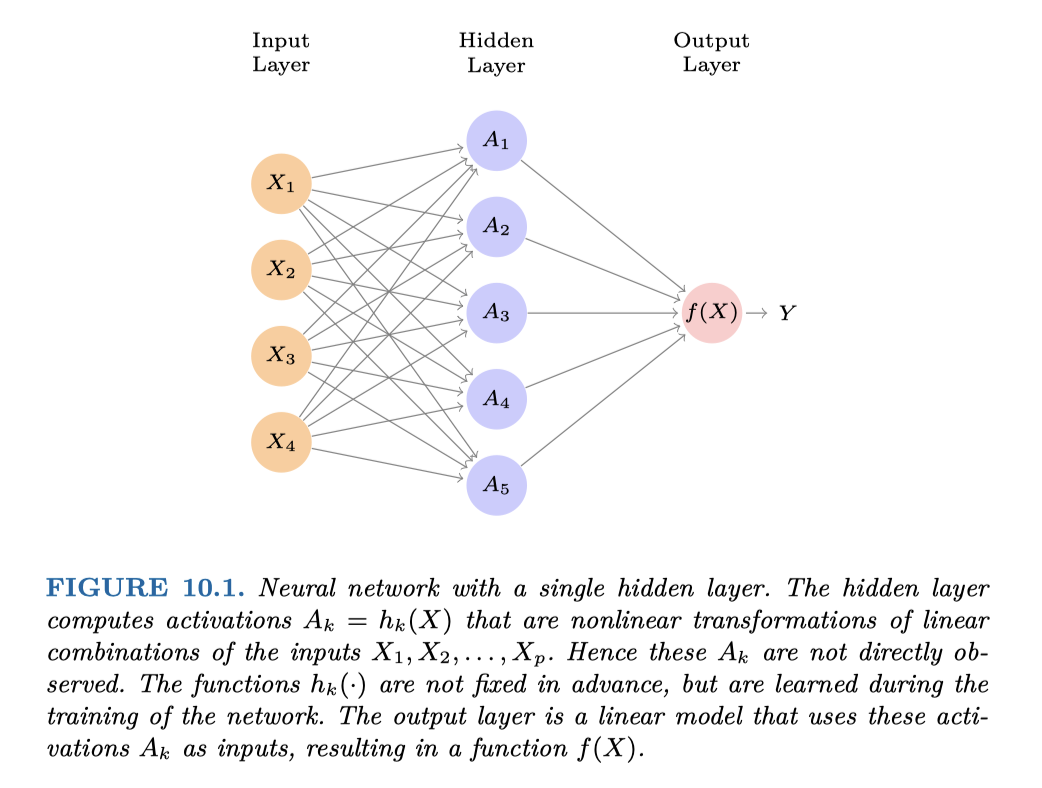
\includegraphics[width=0.75\linewidth]{SLNN.png}
\end{figure}
Input Layer, Hidden Layer, Output Layer, one for each.\\

\textbf{Feed forward}: \\
Start from input layers (features), then apply \textbf{activation functions} within each neurons, and then \textbf{feed it further}.\\

For the output layer, a final function $f(X)$ is applied to all of the values of hidden units (neurons) that are fed to the output layer.\\

Some activation functions: \\
\begin{enumerate}
    \item Sigmoid function: (also known as logit function)\\
    \[\displaystyle g(z) = \frac{1}{1 + e^{-z}}\]\\

    \item ReLU function: (easier for computer since binary cases)\\

    \[g(z) = (z)_+ = \begin{cases}
        0 & \text{if } z < 0\\
        z & \text{otherwise}
    \end{cases}\]
\end{enumerate}

\textbf{Non-linearity} of $\boldsymbol{g(z)}$ is essential.\\


\textbf{Multilayer Neural Networks} (\texttt{MNIST} dataset):

\begin{figure}[h!]
    \centering
    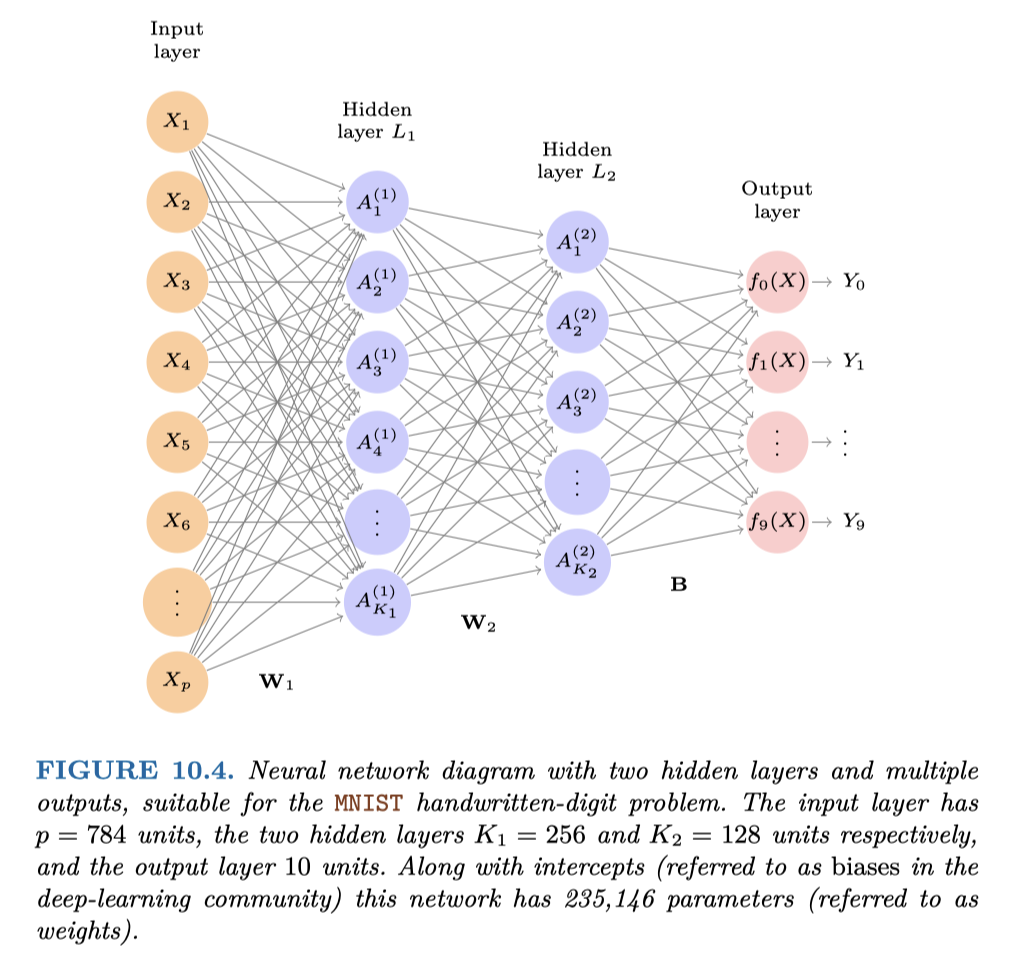
\includegraphics[width=0.75\linewidth]{MLNN.png}
\end{figure}

A fully connected dataset, with the dimension from features $(X)$ feed to the first layer via weight matrix $W_1 = 785 \times 256$ parameters; and from the first to the second layer via weight matrix $W_2 = 257 \times 128$ parameters. (add $1$ to account for the \textit{bias} or \textit{intercept} term)\\

Since we want to have class probabilities, we use \textit{softmax activation function}:\\
\[f_m(X) = P(Y = m | X) = \frac{e^{Z_m}}{\sum_{\ell = 0}^9 e^{Z_\ell}}.\]

$10$ numbers, with each has a non-negative possibility, and all of them sum up to $1$.\\

Estimated via minimization of the negative multinomial log-likelihood:\\
\[-\sum_{i=1}^n\sum_{m=0}^9 y_{im}\log\big(f_m(x_i)\big)\]

\begin{figure}[h!]
    \centering
    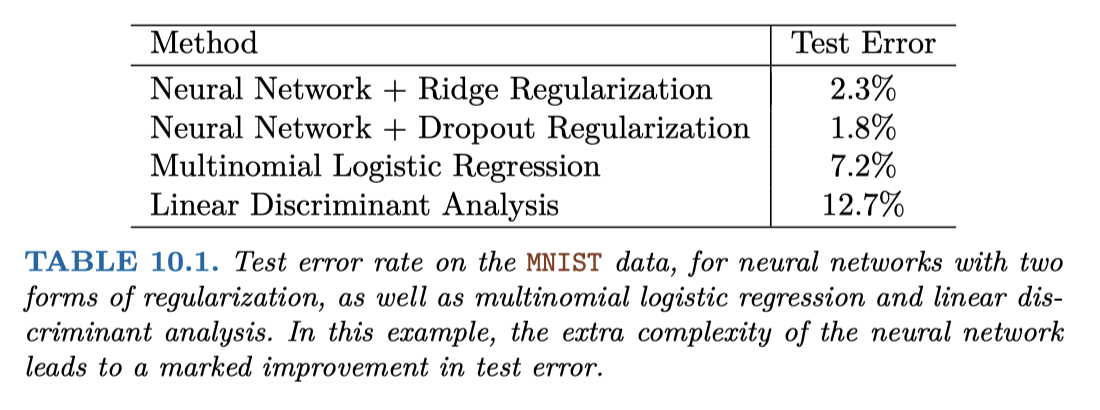
\includegraphics[width=0.75\linewidth]{strategies.png}
\end{figure}

\textbf{What is Dropout?}\\

In essence, silence some nodes randomly.\\

\begin{figure}[h!]
    \centering
    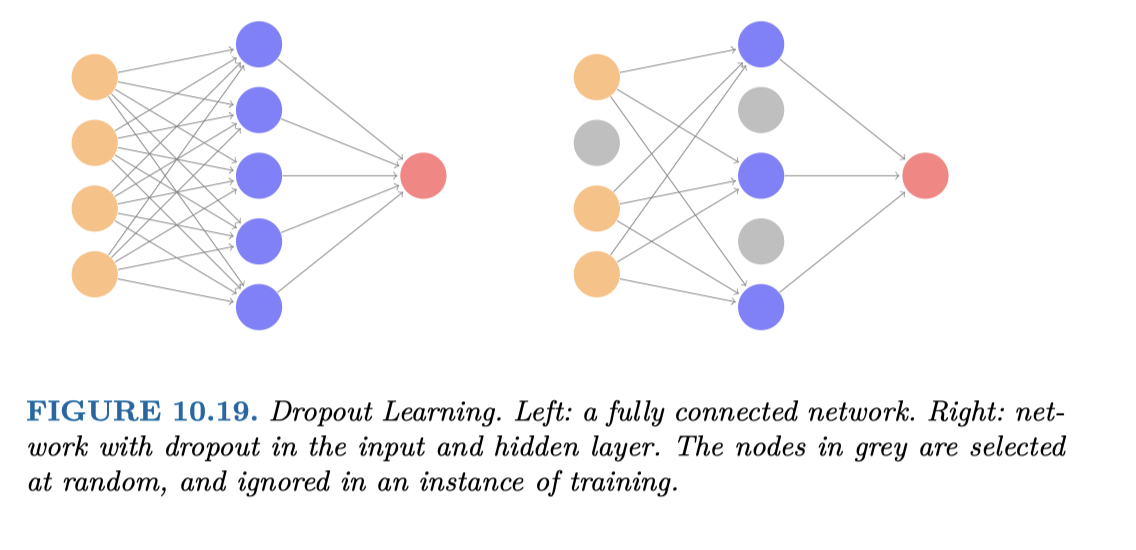
\includegraphics[width=0.75\linewidth]{Drouput.png}
\end{figure}

\textbf{Convolution Neural Networks}: (CNN)\\

Utilizes convolution filters to create extra features from the images. Way better than non-CNN methods for image classification tasks.

\newpage 
\begin{figure}[h!]
    \centering
    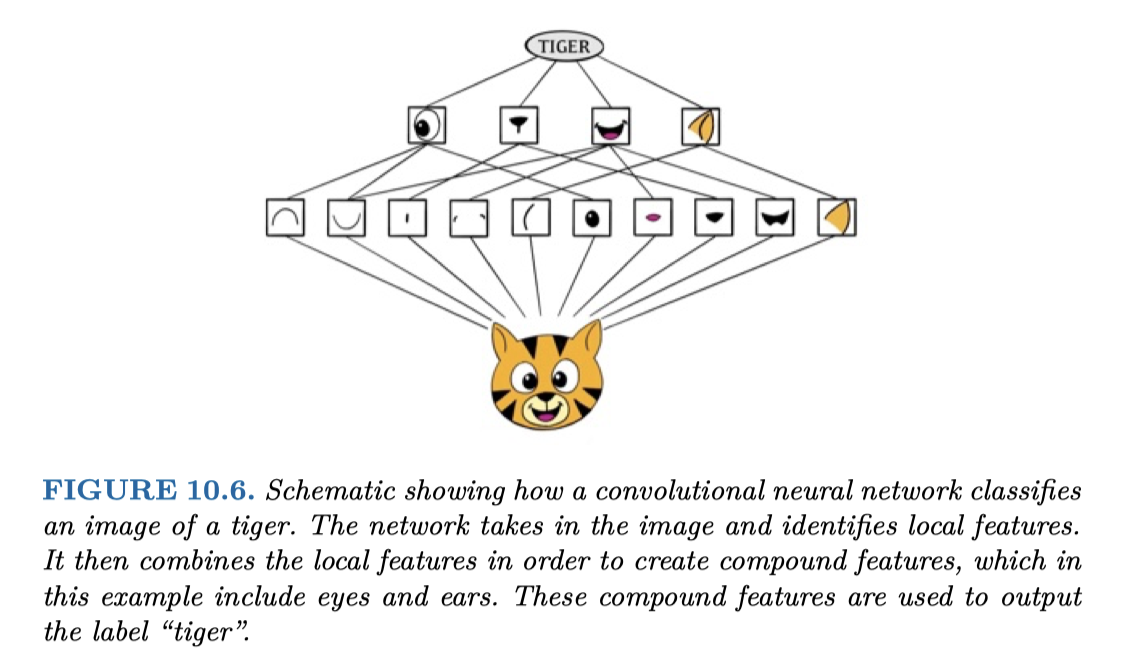
\includegraphics[width=0.75\linewidth]{logistic_CNN.png}
\end{figure}

Convolution filter:\\

\begin{figure}[h!]
    \centering
    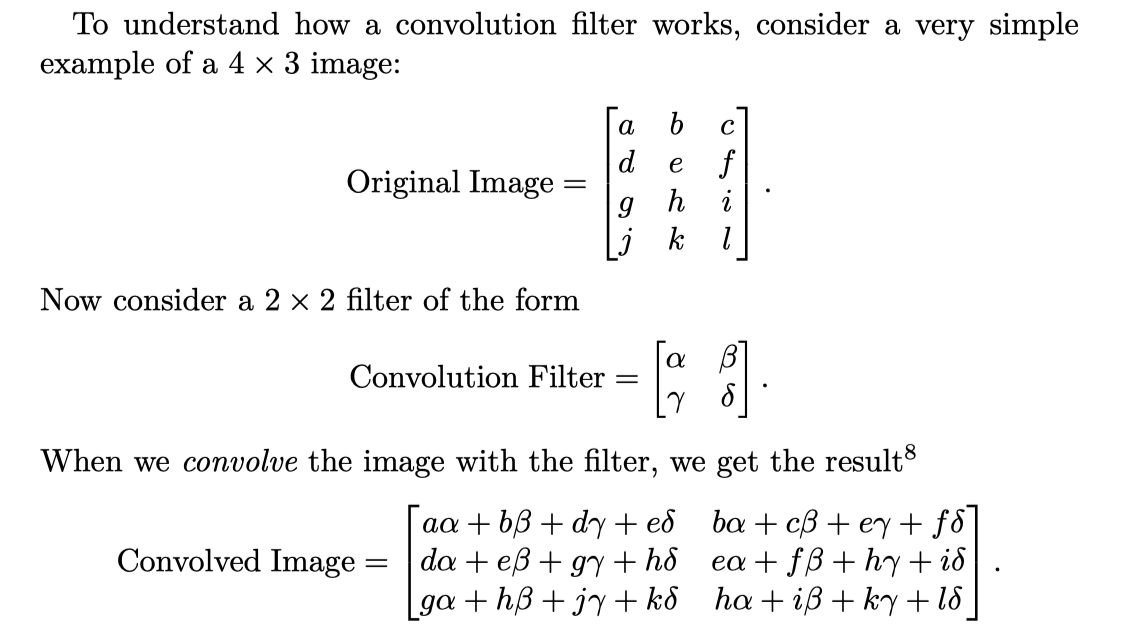
\includegraphics[width=0.75\linewidth]{Convolution.png}
\end{figure}

\end{document}
